\section{Consultar Tratamientos}

Un paciente tendrá una lista con todos sus tratamientos. De esta manera sabrá cuantos y cuáles son sus tratamientos, su estado y la información de estos, como nombre de tratamiento, doctor que expidió, fecha de expedición y medicamentos.

\subsubsection{Procedimiento}
\begin{enumerate}
	
	\item Da clic en el icono \textbf{Tratamientos} de la pantalla \textbf{Menú Principal}.

		\begin{figure}[!htbp]			\hypertarget{fig:mpPacienteTr3}{\hspace{1pt}}
		\begin{center}
			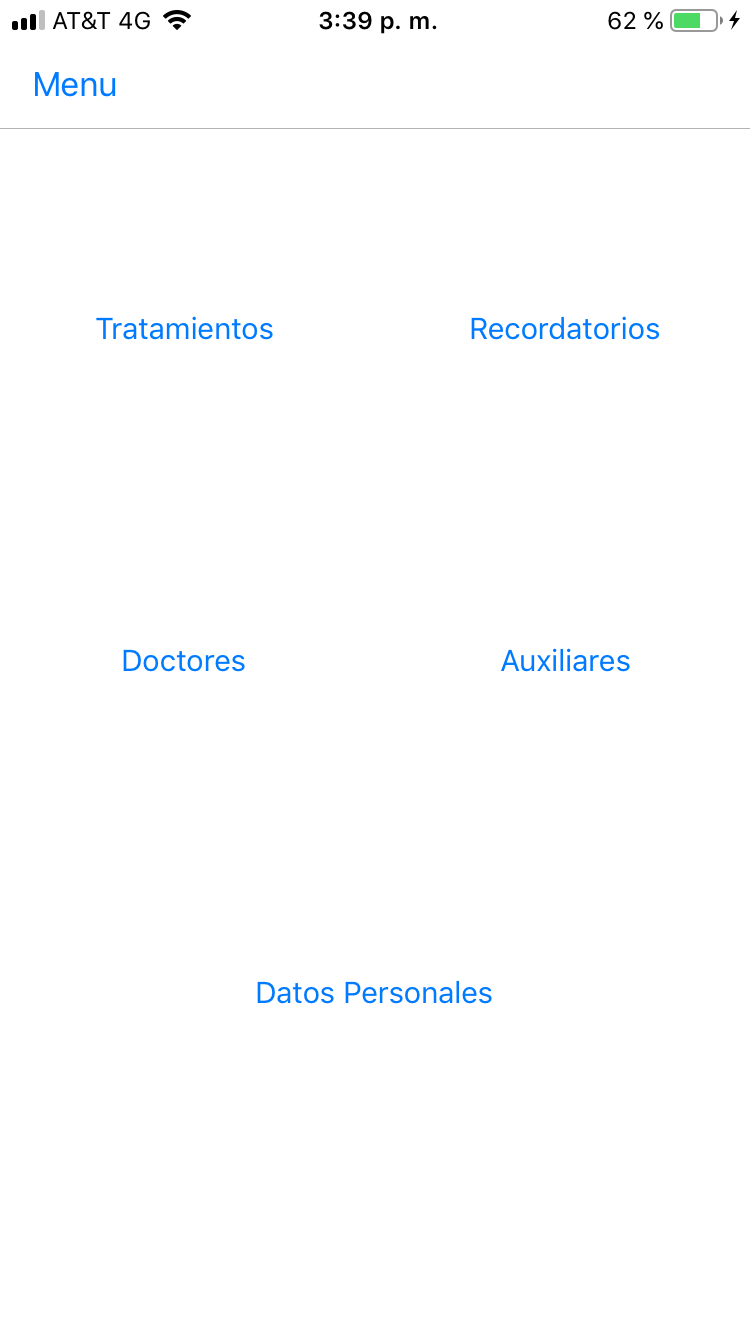
\includegraphics[height=0.4\textheight]{Paciente/ConsultarTratamiento/images/mpPaciente}
			\caption{Menú Principal Paciente}
			\label{fig:mpPacienteTr3}
		\end{center}
	\end{figure}

	\item Se mostrará la pantalla \textbf{Tratamientos}. 
	\newpage
	\begin{figure}[!htbp]			
		\hypertarget{fig:Tratamientos}{\hspace{1pt}}
		\begin{center}
			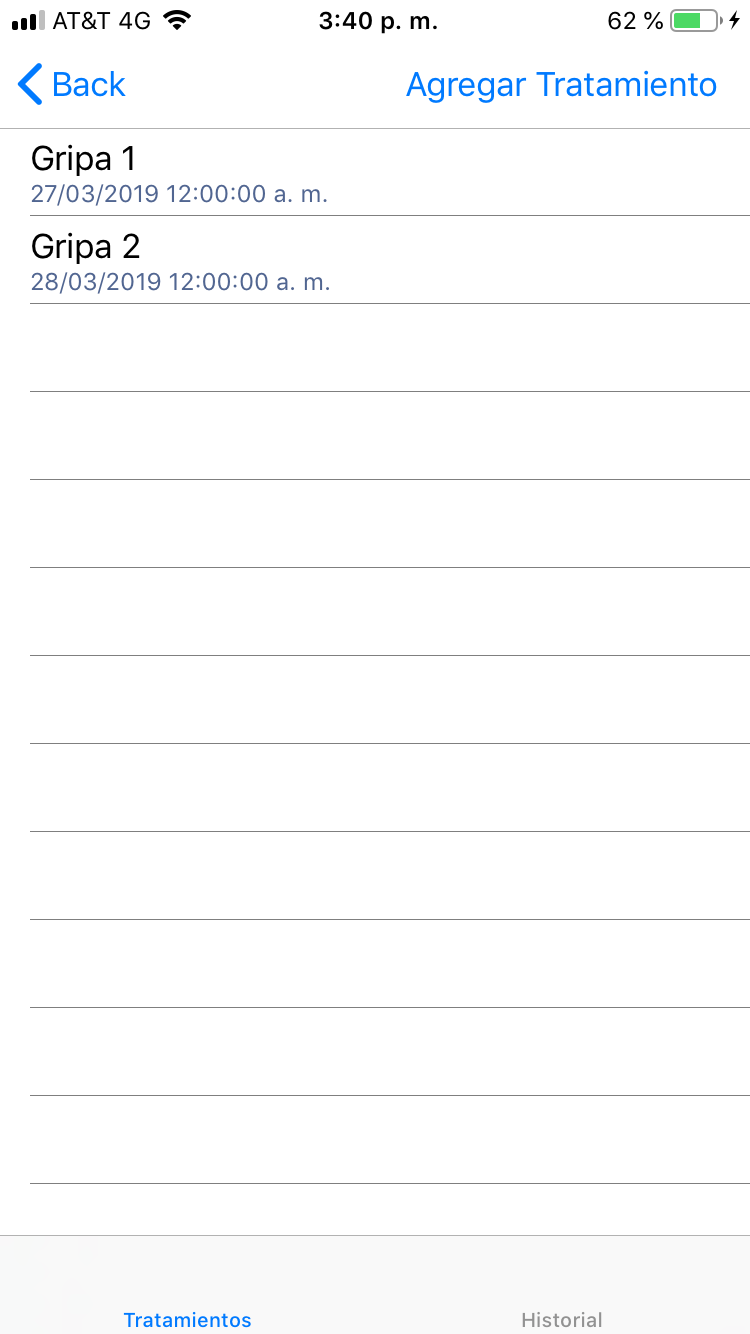
\includegraphics[height=0.4\textheight]{Paciente/ConsultarTratamiento/images/Tratamientos}
			\caption{Tratamientos}
			\label{fig:Tratamientos}
		\end{center}
	\end{figure}

	\item Consulta la información necesaria de tus tratamientos y luego da clic en el botón \textbf{Back} para regresar a la pantalla \ref{fig:mpPacienteTr3} \textbf{Menú Principal.}
	
\end{enumerate}

